%Every piece of package I've acumulated over the last years
%
%
\documentclass[a4paper,12pt]{article}
\usepackage[utf8]{inputenc}
\usepackage{imakeidx}
\usepackage{graphicx}
\usepackage{float}
\usepackage{amsmath}
\usepackage[backend=bibtex,style=verbose]{biblatex}
\bibliography{bibliography}
\usepackage{csquotes}
\usepackage{tcolorbox}
\usepackage{multirow}
\usepackage{caption}
\usepackage{afterpage}
\newcommand\emptypage{
\null
\thispagestyle{empty}
\addtocounter{page}{-1}
\newpage
}
%End of packages
%
%
%
\begin{document}

\title{Pohl's Pendulum}
\author{Gabriel D'Andrade Furlanetto \\ Pablo Hernández Rodríguez }
\maketitle
\pagebreak 
\begin{abstract}
    This paper concerns the Pohl’s Wheel, or Pendulum, experiment conducted by the Mechanic and Wave’s subject from the Physic degree of the University of Salamanca. The oscillations under a damped and driven movement modes will be studied in this document in terms of their frequency, damping coefficient, and amplitude. The experimental data has been obtained by the PHYWE Measure application and, by the calculation forward specified, have been determined the natural and resonant frequency, the damping coefficients and resonant amplitude. Everything with their respective uncertainties.
    As a result, we have been able to discuss and represent the variations in the behaviour of oscillations under different damping coefficients, near resonance and in  stationary state.
\end{abstract}
\pagebreak

\section{Introduction}

\subsection{Objectives}

A harmonic oscillator is a system which traces a sinusoidal movement around its equilibrium due to restoring forces. In this simple situation, its motion is determined by two variables: frequency and amplitude. Despite this being only an idealization rather than a real system, these values, the quantity of oscillations per second and maximum distance from the equilibrium point respectively, are required to study the more complicated systems we will analyze: Damped oscillator, which involves an additional viscous force, and the driven oscillator, which adds an external force.

 These two have their own movement and development in time, therefore in this experiment, we aim to get the constants that allow us to define and predict their evolution. In order to study these abstract systems, we have used Pohl’s Wheel, a torsion pendulum able to reproduce both behaviours, to make measurements that provide us with experimental data for the calculations.

Therefore, the first point of our experiment is the damped oscillator. The objective of our measurements includes the determination of the natural frequency and obtaining the damping coefficient under different voltages, which in a Pohl’s Wheel generates the damping. 

The driven oscillator is the second focus of this experiment. We wait to reach a stationary resonant state of oscillations and, making use of the results obtained previously and the experimental measurements, get the frequency of this phenomenon. We will also investigate the relationship between the amplitude of stationary states and their frequencies. 


\subsection{Theoretical Background}
Our experimental setup is made up of 3 basic components: A torsion pendulum, a copper coil around its lower part that generates a magnetic field, and an electric motor. In essence, the magnetic field will create a magnetic force contrary to the motion of the pendulum\footnote{The precise reason as to why is related to the induction of so-called \textit{eddy currents} as a consequence of Faraday's Law. They are a complex phenomenon that are usually skipped over in elementary texts in Electromagnetism, but luckily the specific case of Pohl's Pendulum is covered in \cite[486]{Zangwill} }, something that will amount to a dampening force, and the motor which will function as a driving force for our system.

As we are working with a rigid solid and not a point particle, it is appropriate to talk about the torques of our system, of which there are three: Firstly, $\Gamma_1$, which comes from the fact that we are working with a torsion pendulum at all\footnote{This can be thought of as the torque analogue to Hooke's Law. A standard treatment is present in \cite[434]{University}}; Another, $\Gamma_2$, originates from the magnetic field we have control over; The last one, $\Gamma_3$, comes from the driving force of our motor.


  \begin{equation}
  \label{momentos}
  \begin{gathered}
   \Gamma_1 = -k\phi \\
    \Gamma_2 = -\eta \dot{\phi} \\
    \Gamma_3 = K_0 \sin(\Omega t)
  \end{gathered}
\end{equation}

Using the elementary relation between torques and angular acceleration, $I \ddot{\phi} = \sum \Gamma_i$ and \eqref{momentos}, we arrive at the equations of motion for our system:

$$I \ddot{\phi} = -k\phi -\eta \dot{\phi} + K_0 \sin(\Omega t)$$

Which can be expressed in a more convenient form by dividing by $I$ and rearranging:

\begin{equation}
\label{forzada}
    \ddot{\phi} + 2\gamma \dot{\phi} + \omega_0^2 \phi= \alpha_0 \sin(\Omega t)
\end{equation}

Where $\gamma = \frac{\eta}{2I}$, $\alpha_0 = \frac{K_0}{I}$ and $\omega_0 = \sqrt{\frac{k}{I}}$, which is the canonical equation for the driven oscillator. The experiment itself is divided in two parts, one with and one without the motor. Therefore, our analysis will concern first the simpler case of the damped and then the general case of the driven oscillator.

\subsubsection{The Damped Oscillator}
If we take $\alpha_0 = 0$ in \eqref{forzada}, we will arrive at the equations of motion for the damped oscillator: 
\begin{equation}
\label{amort}
    \ddot{\phi} + 2\gamma \dot{\phi} +\omega_0^2 \phi = 0 
\end{equation}

There are three different solutions to this differential equation depending on the value of $\gamma$ in relation to $\omega_0$, but we will only work within underdamped oscillations, where $\gamma < \omega_0$. That equation has an analytic and pretty simple to find solution\footnote{Although we won't be going into details on the solution here, a very nice treatment of it is present in \cite[173]{Taylor}}:
\begin{equation}
\label{amortsol}
    \phi (t) = A_0 e^{-\gamma t}\sin(\omega t + \varphi_0)
\end{equation}
Where if $\phi(0) = \phi_0$ and $\dot{\phi}(0) = 0$\footnote{One can find the equations for $A_0$ and $\varphi_0$ even if $\dot{\phi} \neq 0$, but that would make the calculations of the times of return an order of magnitude more difficult. As such, there needs to be care employed in minimizing the initial velocity during the experiments}:
\begin{equation}
\label{IC}
    \begin{gathered}
    \omega = \sqrt{\omega_0^2-\gamma^2}
    A_0 = \frac{\phi_0 \omega_0}{\omega}
    \varphi_0 = \arctan(\frac{\omega}{\gamma})
    \end{gathered}
\end{equation}

As was mentioned, our main experimental goals for this section is determining both $\omega_0$ and $\gamma$ for our system. For the former, we will approximate $\gamma = 0$ when the magnetic field is turned off and directly measure the period of the oscillations, $T$, and use them to find our constant by the elementary relation$\omega_0 = \frac{2\pi}{T}$. 

For the latter, we will need to use some more sophisticated techniques. In essence, we will exploit the fact that we have precise measurements of the points of return of our system at times $t_n$ and values $\phi_n$. We start by stating the trivial fact that, at the return points, $\dot{\phi} (t_n)= 0$ and, trying to apply it by differentiating \eqref{amortsol}:

$$\dot{\phi} (t_n) = -A_0\gamma e^{-\gamma t_n}\sin(\omega t_n + \varphi_0) + A_0 \omega e^{-\gamma t_n}\cos(\omega t_n+ \varphi_0) = 0 $$

Which we can combine with \eqref{IC}:
$$\tan(\omega t_n + \varphi_0) = \frac{\omega}{\gamma}$$
$$\omega t_n + \varphi_0 - 2\pi n = \arctan(\frac{\omega}{\gamma}) = \varphi_0$$

As such, we arrive at our expression for $t_n$\footnote{It's important to note that this is an intermediate step: In the end, we measure $t_n$ and we won't be using this relation anymore}:
\begin{equation}
    \label{tn}
    t_n = \frac{2\pi n}{\omega}
\end{equation}

Finally, if we use the values of $t_n$ of \eqref{tn} in \eqref{amort}, we will obtain the values $\phi(t_n) = \phi_n$ in the return points, which we also measure experimentally. By working through the algebra, one will arrive at:
$$    \left| \phi_n\right| = \left|\phi_0\right| e^{-\gamma t_n} $$

Or, putting it in a more suggestive form for a linear regression:

\begin{equation}
    \label{regrgamma}
    \ln\left|\frac{\phi_n}{\phi_0} \right| = -\gamma t_n 
\end{equation}

\subsubsection{The Driven Oscillator}

The equations of motion for the driven oscillator, \eqref{forzada}, is a non-homogeneous second order ordinary differential equation, and as such, its solution will be the sum of the homogeneous solution (The damped oscillator) and a particular solution. As we had seen, the homogeneous solution goes to 0 as time increases, and as such, we can understand our solution as composed of a transitory part and a stationary part\footnote{The details of this solution are present in \cite[180]{Taylor}}:

\begin{equation}
    \phi(t) = A_0 e^{-\gamma t}\sin(\omega t + \varphi_0) + \beta \sin(\Omega t - \delta)
\end{equation}

Where
\begin{equation}
\label{IC2}
    \begin{gathered}
    \beta = \frac{\alpha_0}{\sqrt{(\omega_0^2-\Omega^2)^2+4\gamma^2\Omega^2}}\\
    \delta = \arctan(\frac{2\gamma\Omega}{\omega^2-\Omega^2})
    \end{gathered}
\end{equation}
In our analysis, we will basically only consider the stationary part of our system (Which dominates the solutions for times $t \gg \frac{1}{\gamma}$). Specifically, as mentioned, we will study the phenomenon of resonance, which happens at a frequency that maximizes the amplitude of our stationary oscillations, a trivial calculus exercise\footnote{For details, \cite[188]{Taylor}}:
\begin{equation}
\label{OmegaR}
    \Omega_R = \sqrt{\omega_0^2-2\gamma^2}
\end{equation}
\begin{equation}
\label{betaR}
    \beta_R = \frac{\alpha_0}{2\gamma \sqrt{\omega_0^2-\gamma^2}}
\end{equation}

Experimentally, we will be measuring the amplitude, $\beta$,  of stationary states near resonance and their frequencies, $\Omega$, for the different values of $\gamma$ corresponding to the different levels of magnetic dampening. With that, we will try to reproduce the curves that are supposed to come out of equation \ref{IC2}, graphed bellow.

\begin{figure}[H]
    \centering
    \caption{Relative amplitude as a function of relative frequency for different values of the damping coefficient}
    \includegraphics[width=12cm]{ilustración.jpg}
    \label{fig:theory}
\end{figure}

\section{Experimental Procedure}

\subsection{Procedure}
In both parts of the experiment, data was collected digitally using PHYWE Measure software and had, thus, minimal human input. However, as will be discussed in more detail during the results and final considerations sections, there were some problems with the sensors and introduced systematic errors into our measurements.

Having said that, this section will be divided into two parts, corresponding to the two different procedures done to collect data from our setup. This will follow the structure of the rest of the lab report, firstly talking about the damped and then the driven oscillator. 

\subsubsection{Damped Oscillator}
To measure $\gamma$, we had need make use of equation \ref{regrgamma}, and, as can be seen there, that means that we had to measure the amplitudes of the points of return as a function of the times of return, or, as was the case, we had to measure the amplitude as a frequency of time and from there extract our desired information.

To do the measurements, we displaced the pendulum by around 100° from its equilibrium position and started to collect data with the correctly configured PHYWE software for 20 seconds. We repeated this 4 times, one for each voltage level that was recommended to us\footnote{That is, at no voltage, corresponding to an approximation of the harmonic oscillator, and at the knob at 4, 6 and 8.}.

At the end, we were left with a large enough data set from where we could extract the desired information with a good amount of precision.

\subsubsection{Driven Oscillator}
Since we wanted to study the phenomenon of resonance, we must begin by finding the resonant frequency, something that is at times easier said than done. In essence, this is a tedious process of moving around the knobs of the driving motor in an attempt to maximize the amplitude of oscillations once the voltage of the damping was set to 0. 

This was a systematic and time consuming process, but once close enough to resonance, we measured the process in PHYWE Measurement for 1 minute. Following that, we repeated the measurements for the different values of damping. 

In order to investigate the relationship between frequency and amplitude, we needed to collect more points. As such, we attempted to repeat this last part for different values of the frequency that were close to resonance. Ideally, we would have done this to at least 2 frequencies above and 2 frequencies below our resonant frequency, but because of time constraints, technical issues and some deeply unphysical curves, we were only able to get one of each. 

\subsection{Measurements}

\subsubsection{Damped Oscillator}\label{damped}
Once finished the experimental procedure,we distinguished the peaks, being the time and amplitude the date required to our calculation. These were the measurements
\newpage
\begin{figure}[h!]
    \centering
    \includegraphics[scale=0.5]{Gráfica 1.PNG}
    \caption{Oscillator: Under natural damping}
    \label{fig:nodamping
    }
\end{figure}
\begin{figure}[h!]
    \centering
    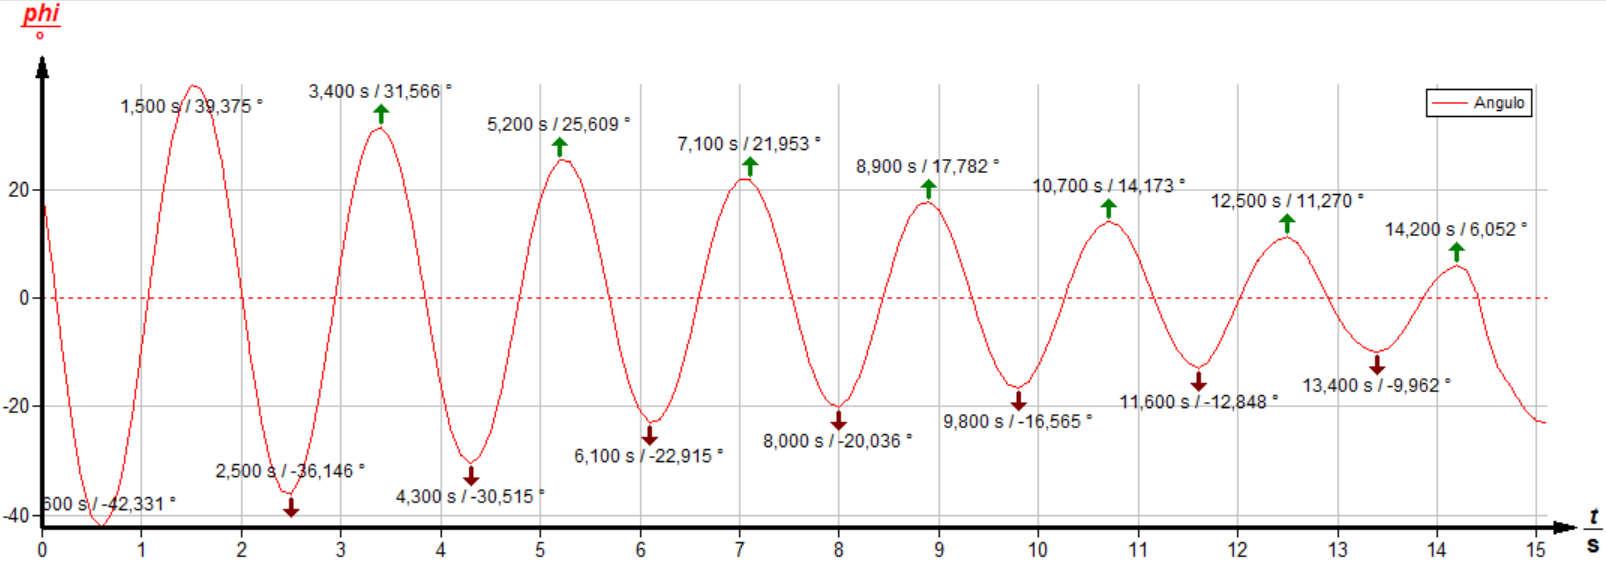
\includegraphics[scale=0.5]{Grafica 2.PNG}
    \caption{Oscillator: Under 4 damping}
    \label{fig:4vdamping
    }
\end{figure}
\begin{figure}[h!]
    \centering
    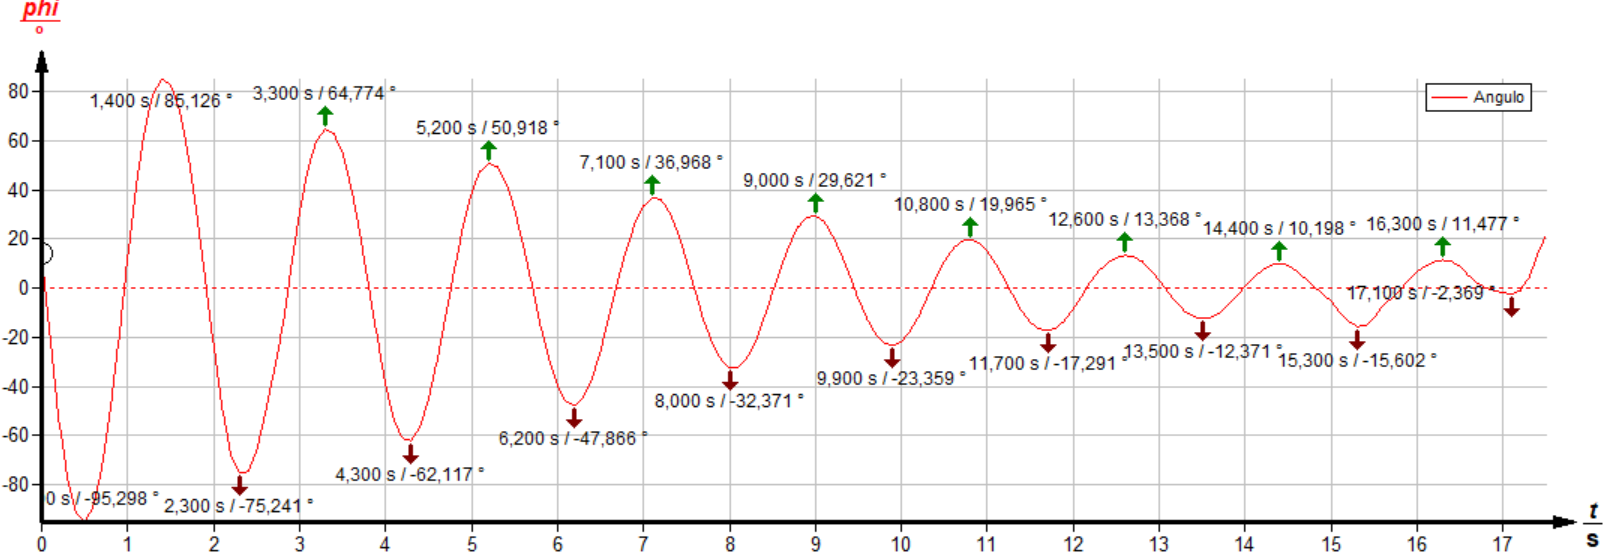
\includegraphics[scale=0.5]{Grafica 3.PNG}
    \caption{Oscillator: Under 6 damping}
    \label{fig:6vdamping
    }
\end{figure}
\begin{figure}[h!]
    \centering
    \includegraphics[scale=0.5]{Gráfica 4.PNG}
    \caption{Oscillator: Under 8 damping}
    \label{fig:8vdamping
    }
\end{figure}
\pagebreak
We decided to dismiss the last results which diverged from the expected behaviour; assuming that under small oscillations the sensor would be imprecise and that the amount of peaks would be enough for the statistical treatment.
Our objective was to study the different damping coefficient, $\gamma$, under the variation of the voltage. In order to that we made use of \eqref{regrgamma} and a linear fit. By another linear fit of the equation \eqref{tn} we will obtain the frequency, $\omega$; both these values allowed us to determine the natural frequency of our oscillator due to \eqref{IC}.

\begin{table}[h!]
    \centering
    \caption{Damping coefficients under different voltages}
    \begin{tabular}{ | c | c | c | c | c | }
    \hline
	& Natural damping & 4V Damping & 6V Damping & 8V Damping  \\
	\hline
	$\gamma (Hz)$ & $0.0744\pm0.0018$ & $0.1101\pm0.0028$ & $0.1623\pm0.0043$ & $0.274\pm0.013$ \\ \hline
	$\omega$(Hz) & $3,628\pm0.048$ & $3,431\pm 0.008$ & $3,515\pm0.062$ & $3,394\pm0.020$ \\ \hline
	\hline
	$\omega_0$(Hz) & \multicolumn{4}{c|}{ $3,628 \pm 0.03$ } \\
	\hline
    \end{tabular}
    
    \label{table:damp}
\end{table}








\subsubsection{Driven Oscillator}\label{driven}

Having collected the full data set for the driven oscillator, we focused our attention on the peaks of our curves, since we wanted to analyze its angular frequency, $\Omega$, and its amplitude, $\beta$. 

To calculate the former, we analyzed the period of each oscillation, that is, the time $T$ it took for the system to get from one maxima to the other, and averaged them out. Because of this, it was very simple to calculate the uncertainty in our measurements\footnote{In this case, we used the simple relation of $u(x) = \sqrt{\frac{var(x)}{n} + \frac{\Delta^2}{12}}$, which is a standard result of uncertainty from a sample measured with limit of resolution $\Delta$.}. Finally, to calculate our desired quantity it was only necessary to employ the elementary relation $\Omega = \frac{2\pi}{T}$ and propagate uncertainties accordingly.

The amplitude of the oscillations is even simpler, since we only must average the absolute value of our peaks and calculate the uncertainty in the same manner as before. In the end, repeating that procedure for different values of damping and frequency:

\begin{table}[h!]
\caption{Amplitudes and frequencies collected from the measurements for different levels of damping. The first row of frequencies represent our best approximation of the resonant frequencies.}
\begin{tabular}{|c|c|c|c|c|}
     \hline
     &Natural damping &  Voltage at 4 & Voltage at 6 & Voltage at 8\\
     \hline
     $\Omega_1$(Hz) & $3.284 \pm 0.013$ &$3.303 \pm 0.010$ & $3.321 \pm 0.008$ & $3.324\pm 0.016$ \\
     \hline
     $\beta_1$(°) & $131.77 \pm 0.91$ & $70.77 \pm 0.69$ & $25.893 \pm 0.099$ & $15.39 \pm 0.18$\\
     \hline
     $\Omega_2$(Hz) & $3.157 \pm 0.016$ & $3.150 \pm 0.039$ & $3.127 \pm 0.022$ & $3.177\pm 0.040$\\
     \hline
     $\beta_2$(°) & $13.61\pm 0.42$ & $12,78 \pm 0.41$ & $11.48 \pm 0.65$ & $11.29\pm 0.58$\\
     \hline
     $\Omega_3 $(Hz) & $3.316 \pm 0.015 $ & $3.335 \pm 0.015$ & $3.344 \pm 0.022$ & $3.340 \pm 0.029$\\
     \hline
     $\beta_3$ (°) & $87.18 \pm 0.27$ & $43.42 \pm 0.31$ & $18.73 \pm 0.29$ & $13.24 \pm 0.44$\\
     \hline
\end{tabular}

\end{table}

With this data at hand, it is possible to illustrate the relationship between frequency and amplitude:

\begin{figure}[H]
    \centering 
    \caption{Amplitude as a function of frequency for the different values of damping.}
    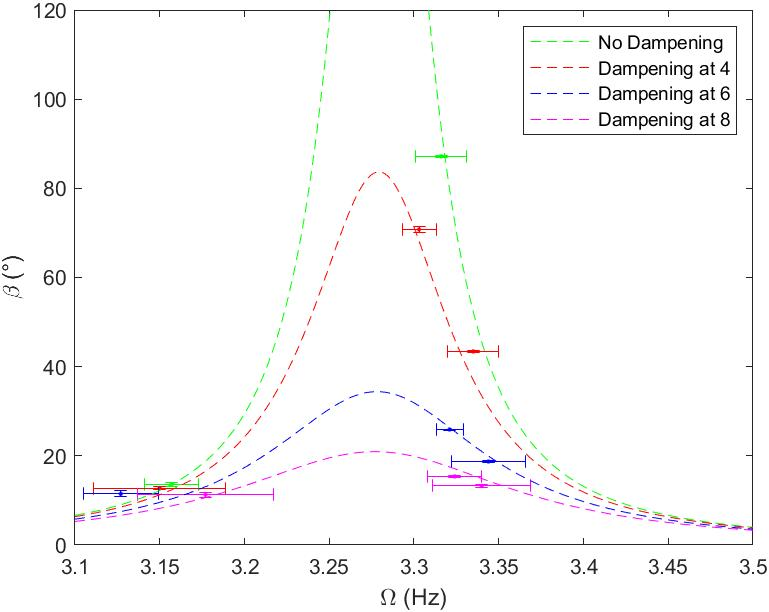
\includegraphics[width=12cm]{forzado.jpg}
    
    The dashed lines are not to be taken as extrapolations of the curve from the data, as there are too few data points to justify anything close to that. Instead, they are there to make the graph more readable.
    \label{fig:forzado}
\end{figure}

As can be seen, this reproduces Figure \ref{fig:theory} very closely, and has the expected behaviour of displaying a maximum at the resonant frequency, followed by monotonic decrease and preceded by monotonic increase. 
%La figura 1 es la regresión lineal en matlab para el amortiguamiento, por si lo necesitases
%
%vale
\section{Results}

Thus far, we have calculated the natural frequency of our oscillator,$\omega_0$, the damping coefficients for the different voltage levels, $\gamma$ in section \ref{damped}, and we have calculated the value of the resonant frequency, $\Omega_R$, and also analyzed the relation between the driven frequency and the amplitude in section \ref{driven}.

Theoretically, these should be complimentary pieces of data, that is, they should agree with one another and give us peace of mind in the accuracy of our results. However, if we start to carry out the calculations, we will find problems. Starting with the case of no damping, using results from table \ref{table:damp}, equation \ref{OmegaR} and standard uncertainty propagation:

\begin{equation*}
    \Omega_{R} = \sqrt{\omega_0^2-\gamma^2} = 3.627 \pm 0.003 Hz
\end{equation*}

And this does not look good: Experimentally, we had found that $\Omega_{Rdriv} = 3.284 \pm 0.013$, which is far enough from that value as to not be contained within our uncertainties, and far enough to generate an almost null amplitude if $\Omega_{R}$ was the actual resonant frequency. 

Repeating this calculation for our different results, we get that:

\begin{table}[]
    \caption{Comparison of the values of the resonant frequencies obtained from the data of the damped and the driven oscillator}
    \centering
    \begin{tabular}{|c|c|c|c|c|}
    &Natural damping &  Voltage at 4 & Voltage at 6 & Voltage at 8\\
        \hline
        $\Omega_{Rdamp}$ (Hz)& $3.627 \pm 0.003$  &$3.625\pm 0.003$ & $3.621\pm 0.003$ & $3.607\pm 0.004$  \\
        $\Omega_{Rdriv}$ (Hz)& $3.284 \pm 0.013$ &$3.303 \pm 0.010$ & $3.321 \pm 0.008$ & $3.324\pm 0.016$
    \end{tabular}
    
    \label{tab:my_label}
\end{table}

Which produces an unacceptable abyss between the values obtained from the collection of data from the damped and the driven oscillator.

Under normal circumstances, these theoretical\footnote{Here we only mean that they are what theory informs us that the data from the damped oscillator should give us} values would be pointed out in Figure \ref{fig:forzado}, but one should observe that they are not even in the limits of the graph; that is, the curve is essentially flat at those values of frequency, certainly not resonant.

All of this conspires to produce an almost certain judgement of the existence of systematic errors during the experiments, which shall be discussed in the last section.

\section{Final Discussion}
In isolation, the results from both the damped and the driven oscillations make sense. However, it should be clear from the last section that together, they are incompatible; The discrepancy of the resonant frequencies and their predicted counterparts are simply too large to be ignored or to be contained within experimental uncertainty, and they signal towards systematic errors that cannot be accounted for using standard statistical methods.

We can merely hypothesize on what their actual sources are, but we are strongly inclined to believe that one of the biggest contributors to this was the sensor itself. We had numerous problems of getting highly unphysical results in our curves\footnote{This ranged from getting a very large negative slope in the curve towards negative infinity to instantaneous jumps of over 70°.} and we infer that, in trying to fix those issues, we may have changed the way in which the device collected data in some way.

However, regardless of the issues above, most of the main results still illustrate the theoretical concepts mentioned in the introduction and, in this limited scope, we were successful in studying oscillatory motion.

\printbibliography

\end{document}
